\documentclass[12pt, titlepage, twoside, a4paper]{report}
\usepackage{geometry}
\usepackage{fancyhdr}
\usepackage{graphicx}
\usepackage{textcomp}
\usepackage{float}
\usepackage{amssymb}
\usepackage{amsfonts}
\usepackage{sidecap}
\usepackage[notes]{biblatex-chicago}
\bibliography{./references/references}
\usepackage{amsmath}
\usepackage[nottoc]{tocbibind}
\graphicspath{ {images/} }
\pagestyle{fancy}
\fancyhead{}
\fancyhead[LO,RE]{Liars, Truth-tellers, and Interactive Identification}
\fancyhead[RO,LE]{Axford, Cairns, Perry}
\fancyfoot{}
\fancyfoot[LE,RO]{\thepage}
\fancyfoot[LO,CE]{Section \thesection}

\title{
{What Kinds of Liars and Truth-tellers Exist, and How Can They Be Identified Through Interaction?} \newline \newline
{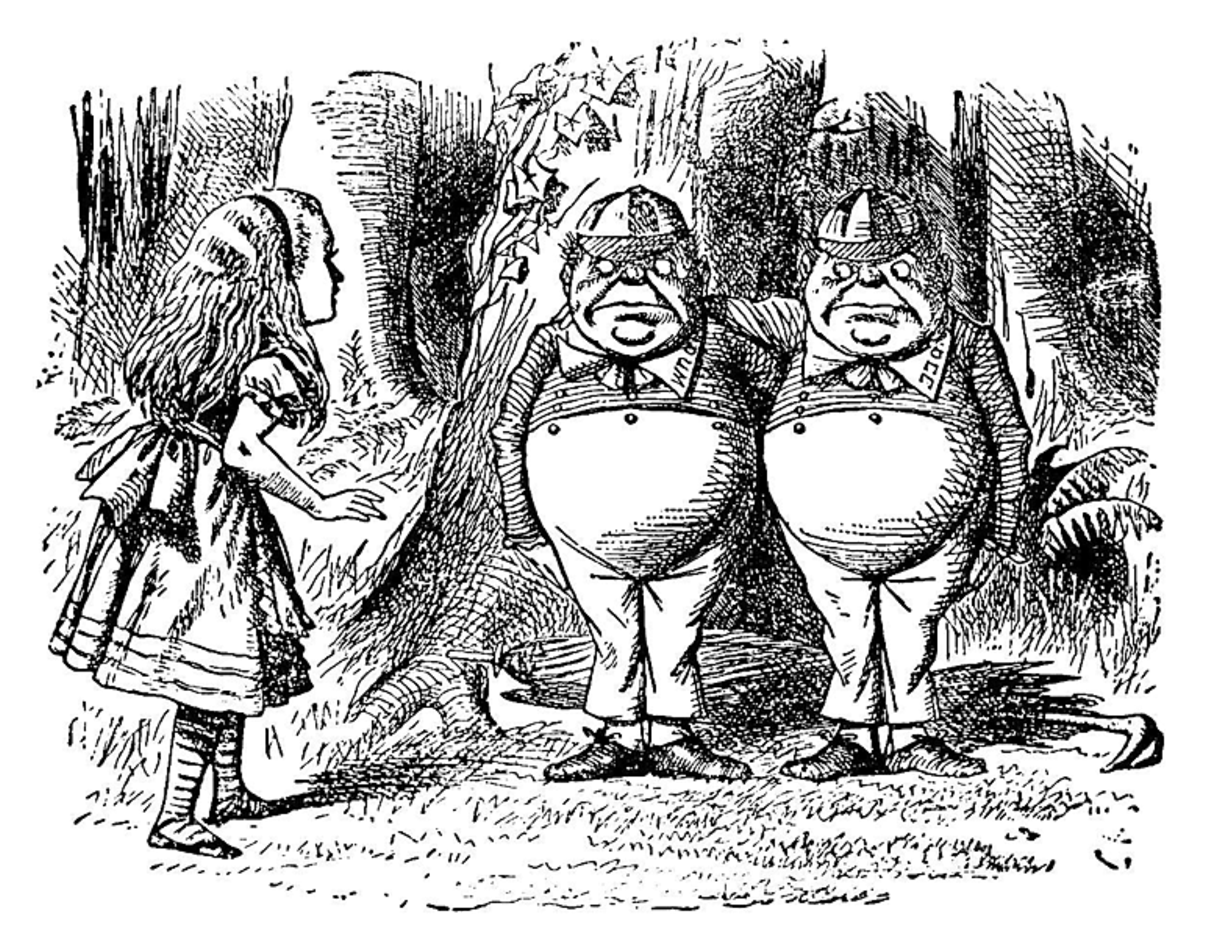
\includegraphics[width=11cm]{alice.eps}}\\
{\large University of Auckland}\\
{\large Philosophy 315}\\
\author{Forrest Axford, Jason Cairns, Emma Perry}}

\newcommand{\true}{$T\text{\textmusicalnote}$}
\newcommand{\false}{$F\text{\textmusicalnote}$}

\begin{document}

\maketitle
\tableofcontents
\newpage
\section*{Abstract}
Truth-telling and lying come in many different forms - we intend to develop a taxonomy through the exploration of some intuitive and counter-intuitive types, and determine how an agent's category can be identified through interaction.

\chapter{Lies with Short Legs and Lies with Long Noses: Introduction \& Preliminaries}

\section{Introduction}
Geppetto identifies two types of lies in \textit{Pinocchio} as ``those with short legs, and those with long noses.'' The \textit{Oxford English Dictionary} prefers to define lying with a bit more clarity – it claims lying is characterized as “[making] a false statement with the intention to deceive.” \autocite{WeinerE.S.C.1989TOEd} Neither the former, nor the latter, nor any other proposed definitions of lying are universally accepted as adequate however.\autocite{sep-lying-definition}\\
This paper utilises epistemic and doxastic logic to investigate the nature of lying and truth-telling. This investigation is conducted through an initial presentation of possible logical definitions of liars and truth-tellers, followed by a look at a few games with a loosely `knights and knaves’-like premise to clarify some points of difference between some possible definitions of lying and truth-telling. A relationship between the justification of the belief an agent holds regarding the statement they are expressing and what type of liar or truth-teller they are is identified and used as a preliminary basis of inquiry into the role belief justification may play in conceptions of lying and truth-telling. Liars and truth-tellers with Gettier Knowledge are considered to further investigate this, and then used as a starting point to examine other types of justified or unjustified liars and truth-tellers. Finally, some concluding remarks and a reflection on the work put forth are presented, along with areas for further work and a bibliography.\\
We first set out a number of key assumptions and limitations embedded within our investigation however; as they are numerous and of critical importance to the underlying logic and premises.

\section{Assumptions, Notation, and Limitations}
The following inquiry is premised upon several key assumptions. 
We assume that lying or truth telling involves: 
\begin{itemize}
\item A statement, $\psi$, which is either a truth or lie 
\item An agent (either a liar or truth-teller) expressing the statement, denoted by \false$\psi$ if the agent is a liar, \true$\psi$ if the agent is a truth teller, or $X \text{\textmusicalnote} \psi$ if it is unknown whether the agent expressing $\psi$ is a liar or truth teller 
\item At least one agent constituting the Audience of the agent expressing $\psi$, denoted by $\mathcal{A}$. We also assume that all liars announcing $\psi$ do so with the intent to deceive $\mathcal{A}$, and that all truth tellers announcing $\psi$ do so without the intent to deceive $\mathcal{A}$. This intent is not included in our subsequent logical formulations of lying and truth telling but is built into all of them via this assumption to avoid repetition. Assumptions regarding the nature of the logic of belief are also built into our analysis.
\end{itemize}

\subsection{The Importance of Intent}
It is worth noting that the speaker’s intent to deceive by expressing $\psi$ is not inherently related to the speaker’s belief in $\psi$. A speaker may both believe [psi] and express [psi] with an intent to deceive – for example, imagine Anita asks Benito:\\
 “Did you see Chidi yesterday?”\\
Benito, who met up with Chidi yesterday for a working lunch in which Benito worked on a project for ETHICS 101 and Chidi worked on a project for PHIL 315, replies:\\
 “I think Chidi’s been working on his project for PHIL 315 all weekend.”\\
 In this case, Benito’s expresses a statement he believes to be true, but does so with an intent to deceive Anita into thinking that he did not see Chidi yesterday.\\
Similarly, a speaker may believe $\psi$ and announce $\neg \psi$ without any intention of deceiving the listener – for example, imagine Aroha says to Brian “Yeah, I totally hate Cherie” sarcastically, assuming that Brian knows that Aroha does not ‘totally hate Cherie’ at all, but rather adores Cherie. The statement is expressed for humorous or sarcastic effect with no intention of deception.\\
These types of cases are excluded from our analysis by our implicit assumption that all lying is done with an intent to deceive, and all truth-telling is done without an intent to deceive.

\subsection{A Note on Belief}
It’s worth noting that the way in which one defines the logic of belief can have a drastic impact on the logic of liars and truth-tellers. If a Lockean conception of belief is used, a belief threshold $\tau \leq \frac{1}{2}$ can result in a speaker expressing a statement which they believe while they also believe its negation. When lying is defined as $(B_{x\tau} \wedge X\text{\textmusicalnote} \neg \psi)$, for example, the speaker may be both lying and not lying simultaneously. This is logically incoherent, and we therefore restrict our analysis to doxastic logics which either are not credence-based or do not allow for a Lockean framework of belief with $\tau \leq \frac{1}{2}$. 
It is also important to note that the divide in the literature concerning doxastic attitudes (whether to consider belief in an all-or-nothing approach, as credence-based, or some combination thereof) results in significant challenges in the development of a consistent, coherent logic of liars and truth tellers – especially in conjunction with the formalization a taxonomy of liars and truth tellers which takes justification into account.\autocite{Buchak2014,Jackson2018,AdamCarter2016,Jackson2018}

\chapter{Liars and Truth-Tellers and Omniscient Beings, Oh My!: Basic Types and Initial Games}
\section{Initial Types of Liars and Truth-Tellers}
To begin our investigation into the concept of lying and truth-telling, we generated several possible logical definitions of liars and truth tellers as per the table below. We identify two of these basic systems of liars and truth-tellers as conceptually interesting and useful.

\begin{table}[h]
\begin{tabular}{lp{9cm}l}
\hline
   & Description                                                                        & Logical formulation                               \\ \hline
1  & Truth-telling as saying something which is true in reality                         & (\true$\psi \to \psi$)                            \\
2  & Lying as saying something which is not the case in reality                         & (\false$\psi \to \neg \psi$)                      \\ \hline
3  & Truth-telling as saying something sincerely                                        & (\true$\psi \to B_T \psi$)                     \\
4  & Lying as saying something insincerely                                              & (\false$\psi \to \neg B_L \psi$)               \\
5  & Lying as saying something believed to be untrue                                    & (\false$\psi \to  B_L \neg \psi$)              \\ \hline
6  & Truth-telling as saying something that is both true in reality and sincere         & (\true$\psi \to (\psi \wedge B_T \psi)$)       \\
7  & Lying as saying something that is both untrue in reality and insincere             & (\false$\psi \to (\psi \wedge \neg B_L \psi)$) \\
8  & Lying as saying something that is both untrue in reality and believed to be untrue & (\false$\psi \to (\psi \vee B_L \neg \psi)$)   \\ \hline
9  & Truth-telling as imparting knowledge                                               & (\true$\psi \to K_T \psi$)                     \\
10 & Lying as imparting what one knows to be false                                      & (\false$\psi \to K_L \neg \psi$)               \\ \hline
\end{tabular}
\end{table}

\section{Identifying Liars and Truth-tellers through an Update Game}
A simple method of discernment between liars and truth-tellers is through the scope of an update game. For each of these games the agents must adhere to four key conditions:
\begin{itemize}
\item An agent must make a statement to begin the game
\item Statements must be made from one agent to at least one other
\item The second agent $x$ is taken as a reliable source by the first agent $a$:\\
$(x\text{\textmusicalnote}_a \psi \to (\psi \wedge K_a \psi))$
\item An agent must make a statement if possible whenever asked (statements can change, but means of truth-telling cannot change)
\end{itemize}

\subsection{Interaction with Alan Truering and Ada Love-Lies}
Let an omniscient truth-teller be an agent named Alan Truering, and an omniscient liar be named Ada Love-Lies\\
If you know an agent is Ada Love-Lies or Alan Truering, what do you require to know the true state of $\psi$? In this game all you require is the update from the agent, and knowledge of their type, to know the true state of $\psi$\\
If Alan Truering states $\psi$, then you know $\psi$, due to:
\begin{align*}
&(T_a \text{\textmusicalnote} \psi \to K_a \psi)\\
&(K_x K_a \psi \to \psi)
\end{align*}
The proof of this is as follows:
\begin{align*}
&1. \quad (KK_a \psi \to \psi) \quad \quad 											&\text{Hypothesis}\\
&2. \quad (K_a \psi \to \psi) 														&\text{Facticity}\\
&3. \quad (K(K_a \psi \to \psi)) 													&\text{Necessitation}\\
&4. \quad (KK_a \psi \to K_a \psi) 													&\text{Translates across implication}\\
&5. \quad (K \psi \to \psi) 															&\text{Facticity}\\
&6. \quad (((p \to q) \wedge (q \to r)) \to (p \to r)) 								&\text{Tautology}\\
&7. \quad ((KK_a \psi \to K \psi) \wedge (K \psi \to \psi)) \to (KK_a \psi \to \psi)) 	&\text{Substitution}\\
&8. \quad ((KK_a \psi \to K \psi) \wedge (K \psi \to \psi) 							&\text{4,5, Conjunction}\\
&9. \quad (KK_a \psi \to \psi) &\text{7,8, Modus Ponens}
\end{align*}
The same is true for Ada Love-Lies by simply negating her statement.

\subsection{Identification of Alan Truering and Ada Love-Lies}
What if you are presented with an agent $a$, who is either Alan Truering or Ada Love-Lies, but you do not know which?\\
This question is answered by the simple game that presupposes your knowledge of the true state of $\psi$ during the agent's announcement.\\
If $\psi$ is true and the agent announced $\psi$ then you know the agent is Alan Truering. If $\neg \psi$ is true and the agent announces $\psi$ then you know you are dealing with Ada Love-Lies.
This entails the following model, with $x$ as "you", the audience:
\begin{figure}[h!]
  \centering
  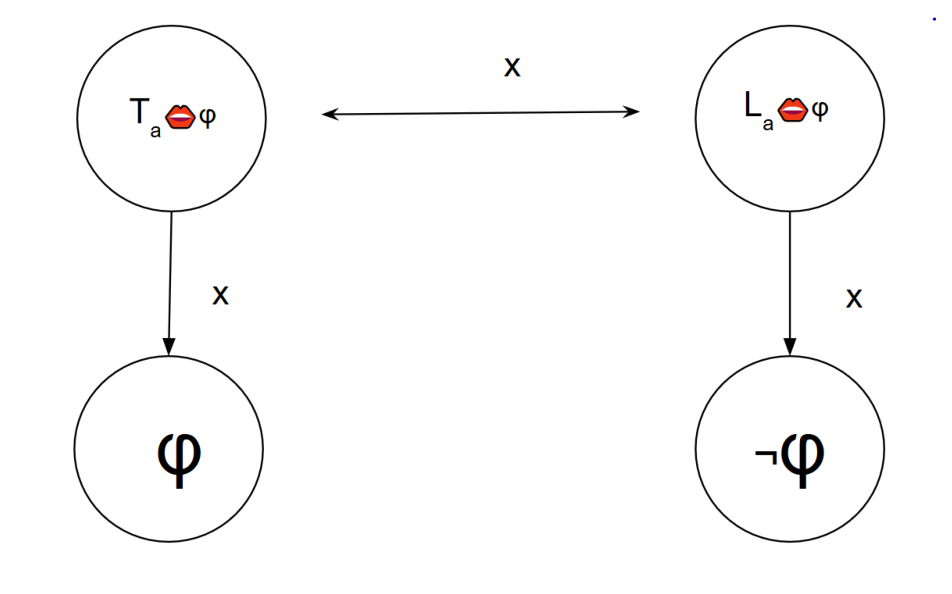
\includegraphics[width=0.5\textwidth]{slide10.eps}
  \caption{Initial space}
\end{figure}\\
\begin{figure}[h!]
  \centering
  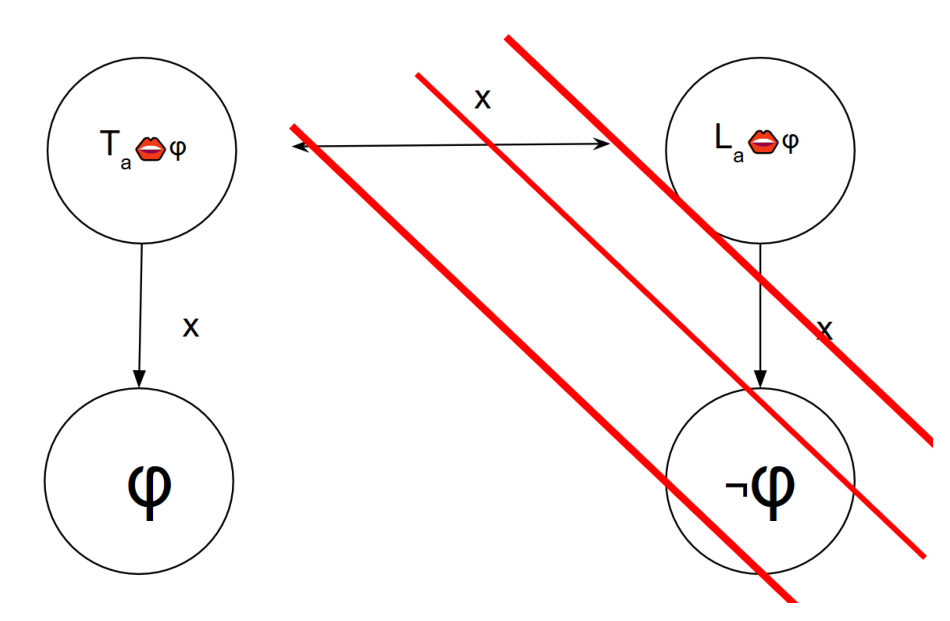
\includegraphics[width=0.5\textwidth]{slide11.eps}
  \caption{After updating with $\psi$}
\end{figure}
\newpage
\section{Sincere and Insincere Men}
So far this game as appeared straightforward, as in each instance there only exists one possible relationship between the agent's statement and the true state of $\psi$ in the world.\\
Now instead of assuming that you must know $\psi$ in order to be a truth teller, consider instead if all that is required to be a truth teller is to believe $\psi$, as per types 3,4, and 5, with liars being defined equivalently.\\
Unlike omniscient liars and truth-tellers, you cannot identify if someone is sincere or insincere based purely off whether their statement is true in reality.\\
\\
Omniscient Truth-teller:
$$((T_a \text{\textmusicalnote} \psi \to K_a \psi)\to \psi)$$
Sincere Men:
$$((T_a \text{\textmusicalnote} \psi \to B_a \psi)\nrightarrow \psi)$$ \\
Simply put, it is possible for people to have incorrect beliefs.

\subsection{Identification of Sincerity}
If we now use the same framework for our game as we have had previously then we are able to identify if an agent is sincere or insincere;\\
Once the agent $a$ makes their claim 
$$a\text{\textmusicalnote} \psi$$
Then if you know $\psi$, all you need to do is update $a$ to $\psi$.\\
If $a$ knows that all updates are true updates $K_a<!\psi >$
\begin{align*}
&K_a \psi\\
&K_a \psi \to B_a \psi\\
&B_a \psi
\end{align*}
Knowing they now have a belief in $\psi$, if you ask them to repeat their statement they will have to respond in specific ways.\\
A sincere man will always state $a \text{\textmusicalnote} \psi$ as they now believe $\psi$\\
An insincere man will always state $a \text{\textmusicalnote} \neg \psi$ as they now believe $\psi$ with $\tau = \infty$ and as such unless they have a threshold of $0$, they will $\neg B_a \neg \psi$

\section{A 4-Player Game}
%NEED WORK ON FORREST SECTION - SEE QUESTION MARKS (?)
Finally, we look at a game in which the agent can exist in four possible states. The agent can be either:
\begin{itemize}
\item Alan Truering (omniscient truth-teller)
\item Ada Love-Lies (omniscient liar)
\item Sincere man
\item Insincere man
\end{itemize}
If the agent announces $\psi$ you are unable initially to distinguish which state they are in, as per the following model:
\begin{figure}[h!]
  \centering
  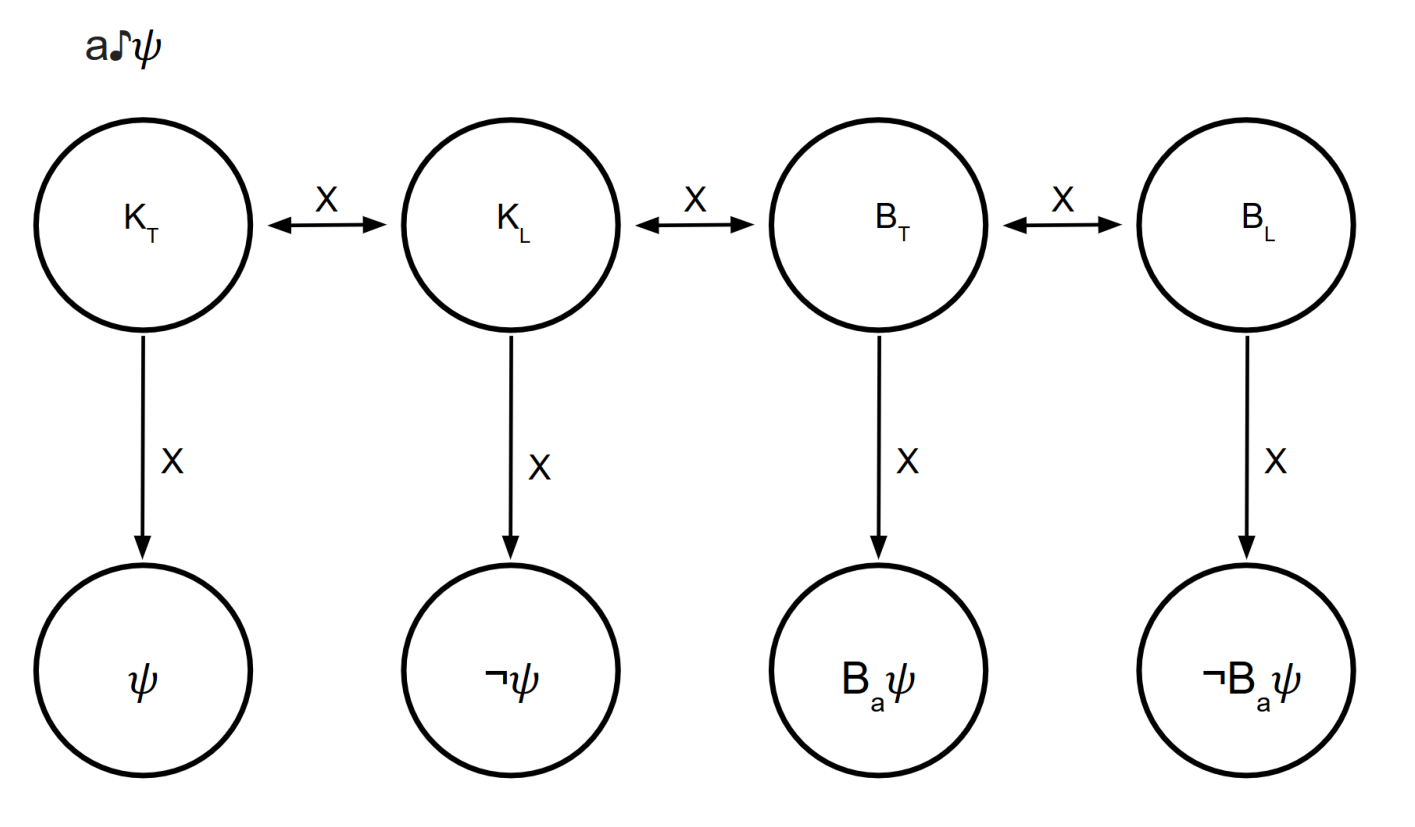
\includegraphics[width=0.5\textwidth]{slide40.eps}
  \caption{Before $a \text{\textmusicalnote} \psi$}
\end{figure}

However, if you come to know $\psi$ to be true then you can eliminate Ada Love-Lies from the possible states of $a$ due to her defining proposition: 
$$(K_L \text{\textmusicalnote} \psi \to \neg \psi)$$
Based on the following derivation:\\
\begin{align*}
&(K_L \text{\textmusicalnote} \psi \wedge \psi )\\
&(K_L \text{\textmusicalnote} \psi )\\
&\psi \\
&(K_L \text{\textmusicalnote} \psi \to \neg \psi )\\
&\neg \psi \\
&\times
\end{align*}\newline \newline \newline
With the following model:\newline
\begin{figure}[h!]
  \centering
  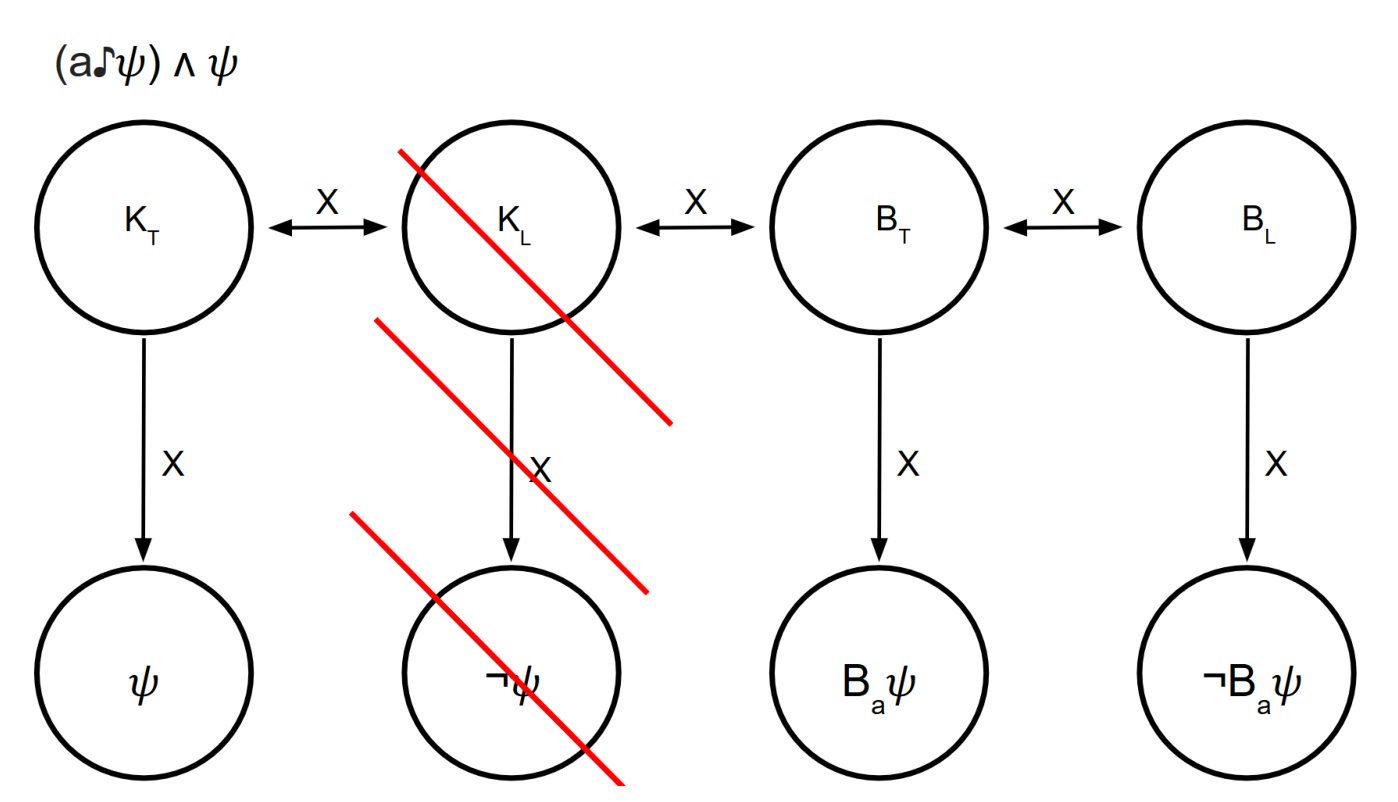
\includegraphics[width=0.5\textwidth]{slide41.eps}
  \caption{After $a \text{\textmusicalnote} \psi$}
\end{figure}\newline
The same format can be used to eliminate Allan Truering if you know $\neg \psi$.\\
\begin{figure}[h!]
  \centering
  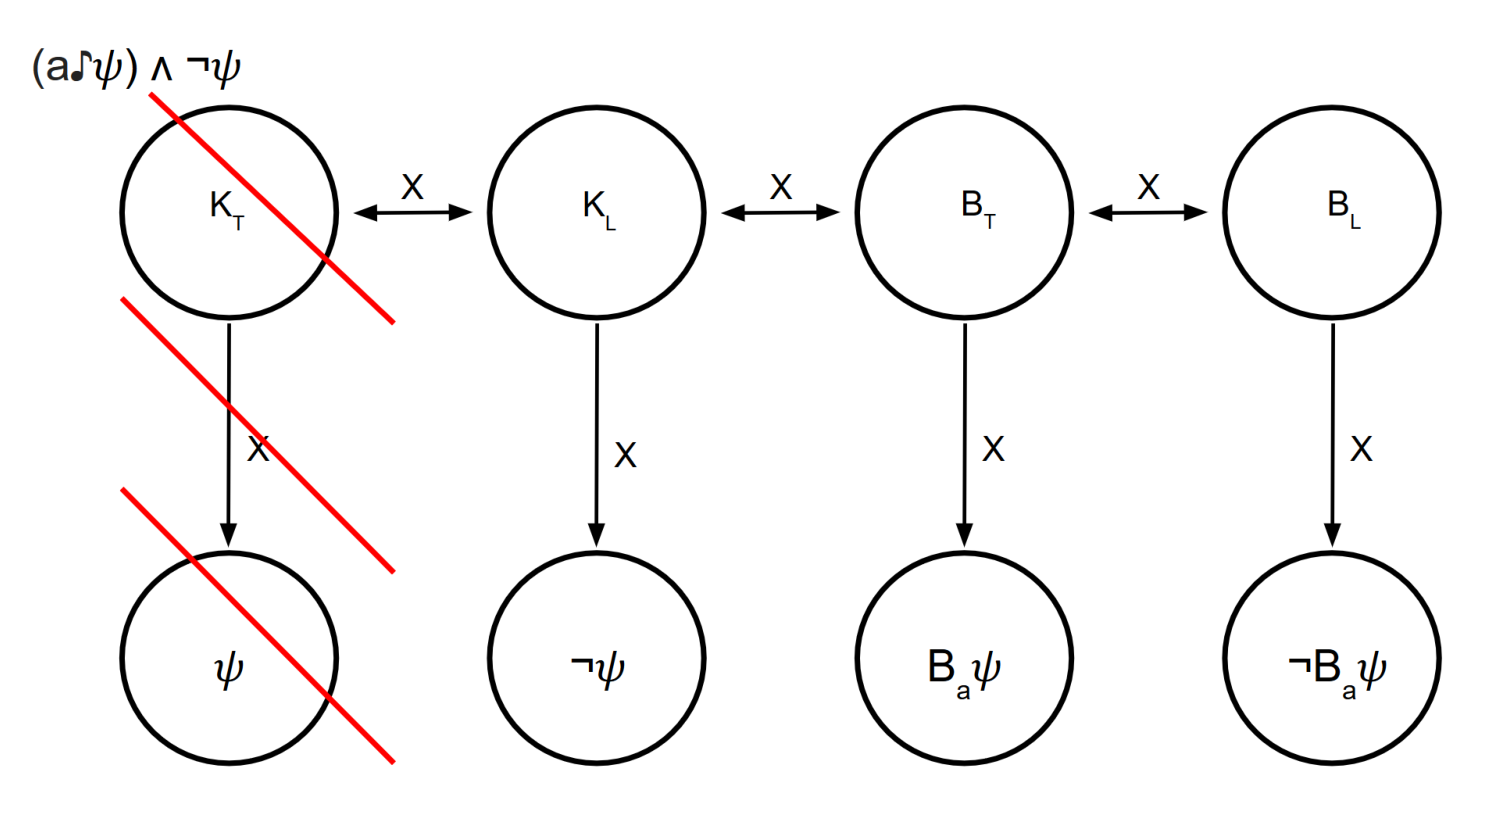
\includegraphics[width=0.5\textwidth]{slide42.eps}
  \caption{After $a \text{\textmusicalnote} \psi$}
\end{figure}\newline
Now with the knowledge of $\psi$, you must discern between Alan Truering and the sincere and insincere men.\\
To do this, you must make an announcement. However, unlike the case in which you are restricted to sincere and insincere men you mus not announce $\psi$ - if you do then $\psi$ becomes public knowledge, thereby allowing the sincere man to hold knowledge of $\psi$, making them indistinguishable from Alan Truering.\\
Instead, announce a simple conjunction:
$$(\psi \to K\psi)$$ 
Each agent will evaluate this statement with relation to their own type.\\
For both sincere and insincere men who are simply evaluating $\psi \to K\psi$ as one normally would, they would correctly identify that $\psi \to K\psi$ does not hold as it is possible to have $\psi$ in the world without knowing $\psi$\\
Thus if the agent is sincere they will believe the statement false and announce $\neg \psi$ as such. 
$$(B_T \text{\textmusicalnote} \neg (K \psi \to K \psi))$$ \\
An insincere man will also believe $\neg \psi$ to be false and as such will not believe it to be true. Therefore they will anounce it to be true as they will announce what they do not believe. i.e. $\psi \to K\psi$\\
However, in the cases for both omniscient states, where this announcement does not follow the same course. For both omniscient states, the agents will know $\psi$ to be true($K\psi$). As the consequent is true, the implication holds true regardless of the antecedent. Therefore for them, $\psi \to K\psi$.
$$K_T\text{\textmusicalnote} (\psi \to K\psi)$$
However, Ada Love-Lies will announce the negation of what they know to be true, therefore;
$$K_L\text{\textmusicalnote} \neg (\psi \to K\psi)$$
We have the following model representations. Note: $\psi$ is in these cases true, so Ada Love-Lies has already been ruled out. Either of the following two models hold; 
\begin{figure}[h!]
  \centering
  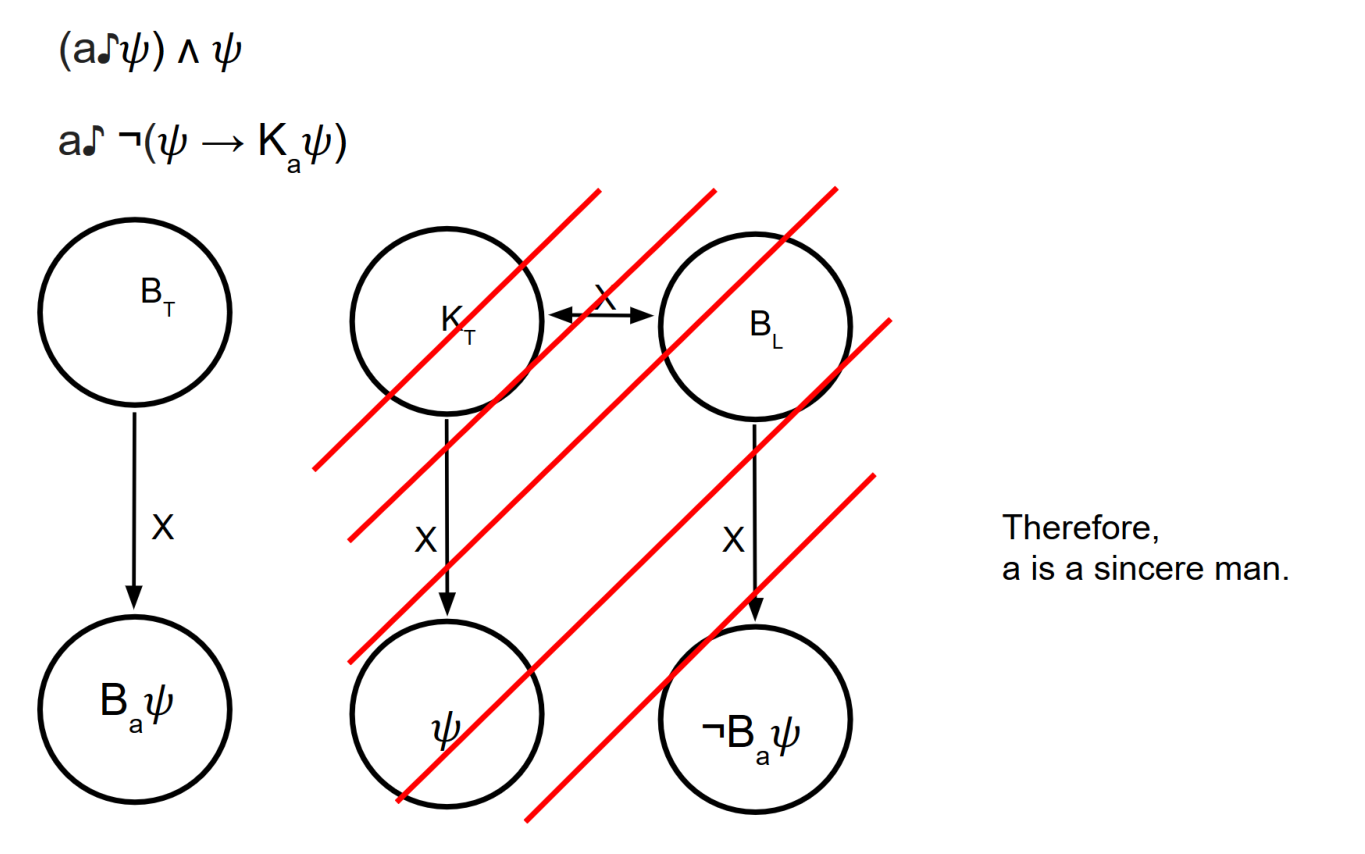
\includegraphics[width=0.5\textwidth]{slide43.eps}
\end{figure}
\begin{figure}[h!]
  \centering
  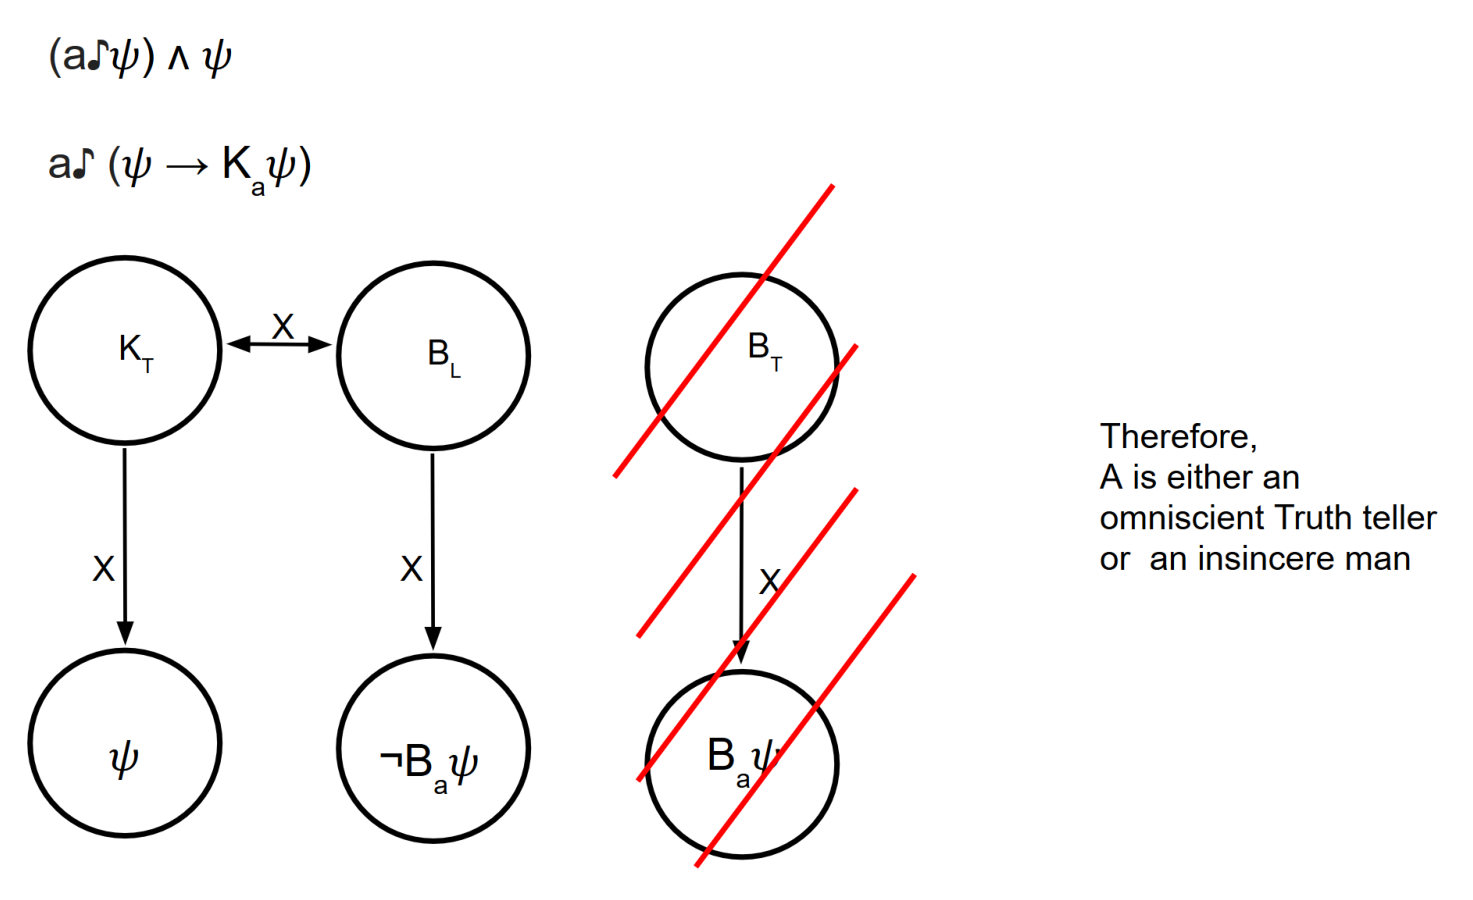
\includegraphics[width=0.5\textwidth]{slide44.eps}
\end{figure}
\newline \newline \newline \newline \newline \newline \newline \newline \newline
Now depending on the response, you can either stop there, as if they respond with $\neg (\psi \to K\psi)$ they can only possibly be the sincere man (as Ada Love-Lies has already been ruled out)\\
If they announce $(\psi \to K\psi)$ to be true, you know the agent to either be Alan Truering or an insincere man.\\
To differentiate between them, simply update the agent to $\psi$.
$$X\text{\textmusicalnote}_a \psi \to (\psi \wedge K_a \psi)$$
To this Alan Truering will announce that $\psi$ is still true. However, the insincere man will have to change his announcement.
$$(((K_a \psi \to B_a \psi ) \to \neg B_a \psi) \to a \text{\textmusicalnote} \neg \psi)$$
If $a$ announces $\psi$, they are Alan Truering, and if $a$ announces $\neg \psi$, they are the insincere man. These steps still work with $\neg \psi$ in the world by simply replacing all instances of $\psi$ with $\neg \psi$ in announcements and eliminating Alan Truering rather than Ada Love-Lies, prior to announcement.

\chapter{Think It Over, Think It Under: Justification and Gettier Types}
\section{Belief, Justification, and Knowledge}
A justified belief may be thought of as a belief $\psi$ that is evidenced by a belief that there exists some $\phi$ such that $(\phi \to \psi)$ holds true and a belief in $\phi$. Let $J_X\psi$ signify that X has a justified belief in $\psi$ – that is:
$$\vdash J_X\psi \leftrightarrow (B_X \psi \wedge B_X(\psi \to \psi) \wedge B_X \phi)$$ 
Then we say X has a justified true belief in $\psi$ if, and only if $J_X\psi \wedge \psi$ holds true in the actual state of the world. Conversely, X has a justified false belief in $\psi$ if, and only if $J_X\psi \wedge \neg \psi$ holds true in the actual state of the world. 
We prove knowledge of $\psi$ implies a justified true belief in $\psi$:

\begin{table}[h]
\begin{tabular}{lll}
1  & $K_X\psi$                                  & Assumption                            \\
2  & $\vdash K_X\psi \to B_X\psi$               & Belief Necessitation                  \\
3  & $\vdash K_X\psi \to \psi $                 & Facticity                             \\
4  & $K_X(K_X\psi \to \psi  )$                  & 3, Epistemic Necessitation       \\
5  & $B_X(K_X\psi \to \psi )$                   & 2, 4, Predicate Logic           \\
6  & $K_XK_X \psi$                              & 1, Positive Introspection        \\
7  & $B_XK_X\psi $                              & 6, Belief Necessitation          \\
8  & $B_XK_X\psi \wedge B_X(K_X\psi \to \psi )$\qquad \qquad \qquad \qquad \qquad \qquad & 5, 7, Predicate Logic           \\
9  & $B_X\phi \wedge B_X(\phi \to \psi)$        & 8, Substitution                  \\
10 & $J_X\psi$                                  & 9, Justification Definition, PL \\
11 & $\psi$                                     & 1,3, Predicate Logic            \\
12 & $J_X \psi \wedge \psi$                     & 10, 11, Predicate Logic         \\
13 & $K_X\psi \to (J_X\psi \wedge \psi )$       & 1 - 12, Predicate Logic         
\end{tabular}
\end{table}

While knowledge of $\psi$ thus implies a justified true belief in $\psi$, a justified true belief in $\psi$ does not imply knowledge of $\psi$. In the game in \textsection 2.4, an agent with a justified true belief, an agent with a justified false belief, and an agent with an unjustified true or false belief will all behave as sincere or insincere agents (depending on their intent to deceive) unless they have knowledge of $\psi$ – so the above game only distinguishes between agents with and without an intent to deceive and between agents who satisfy one specific case of justified true belief (knowledge) and all other agents. There would seem to be value in gaining a better understanding of justification's role in possible definitions of truth-telling and lying, as the notion of justification seems to have some sort of relationship between the actual state of the world and an agent's set of beliefs.\\
Relationships between the actual state of the world and an agent's set of beliefs are of interest in our investigation of the concepts of lying and truth-telling as they would seem to be a strong initial point for a conceptual analysis that takes the effects of lying and truth-telling on a social network into account. To conduct such an analysis is largely outside the scope of this paper, but the initial concept of justification is explored through an analysis of liars and truth-tellers with Gettier Knowledge – a special case of justified true belief in one proposition built upon a false belief in another – and then by negating the definition of agents with Gettier Knowledge to see if any further insight can be gained.  Ultimately, this exploration of the negated definition of agents with Gettier Knowledge is concluded to be too diffuse to provide useful insights but could provide a framework within which more specific cases of justified and unjustified belief and their relationship to lying and truth-telling can be explored. 

\section{Agents with Gettier Knowledge}
\begin{table}[h]
\begin{tabular}{lp{6cm}p{8cm}}
\hline
   & Description                                                 & Logic                                                                                                           \\ \hline
11 & Gettier Truth-tellers announce truth, for the wrong reasons & (\true$\psi \to ((\neg \phi \wedge \psi ) \wedge B_\tau (\phi \to \psi ) \wedge B_\tau \phi)$)       \\
12 & Gettier Liars announce falsity, for the wrong reasons       & (\false$\neg \psi \to ((\neg \phi \wedge \psi ) \wedge B_\tau (\phi \to \psi ) \wedge B_\tau \phi)$) \\ \hline
\end{tabular}
\end{table}
Based on Van Bentham's notion of a Gettier Truth-teller\autocite{BenthemJohanvan2010Mlfo}, consider a Gettier Truth-teller defined as such; Gettier Truth-tellers announce truth, sincerely, but based on false evidence. They announce $\psi$, which is true in reality, based on some evidence $\phi$, which is false in reality. They make this based on a modus ponens implication of $(\phi \to \psi)$, the only falsity being their belief in $\phi$, which is false.\\
Gettier Liars exist in a similar manner, the primary difference being that they seek to deceive, negating the truth, which they succeed in, but based on evidence that is false.

\section{Gettier Interactions}
From their announcement of $\psi$ as well as your knowledge that they believe $\phi$ falsely, then due to the nature of implication, $(\phi \to \psi)$ holds regardless of the truth value of $\phi$, due to $\psi$ being true. Therefore you can't immediately conclude that they are a Gettier Truth-teller - they may be entirely generic.\\
In order to ascertain them as Gettier, truthfully announce that their (false, but not necessarily known to you) antecedent $\phi$ leads to the negation of a different (true, but not known to them as true) consequent $\rho$,  giving the common knowledge $(\phi \to \neg \rho)$, and they should then be able to make the announcement of their belief in the negation of the (true) consequent $\rho$, i.e. $\neg \rho$, which you know to be a falsehood. This can be modelled as:\\
\begin{figure}[h]
  \centering
  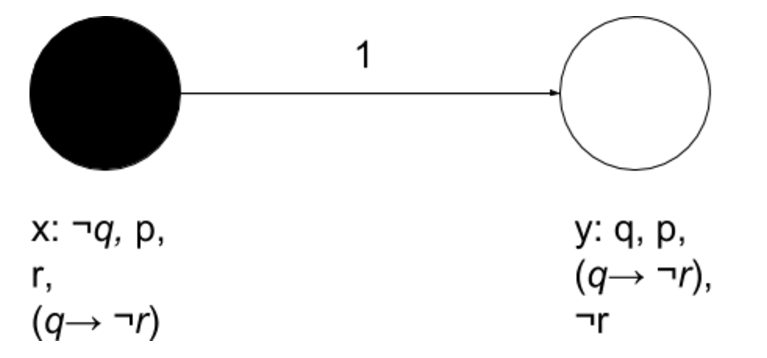
\includegraphics[width=0.5\textwidth]{gettiermodelbase.eps}
  \caption{Plausibility model}
\end{figure}\\
Gettier Liars Interaction is symmetrical to Gettier Truth-tellers - this is not a unique property  of Gettier announcers, however it is worth noting that symmetry isn't common to all types, such as 3,4,5
\newpage
\subsection{State Plausibility Models}

\begin{figure}[h]
  \centering
  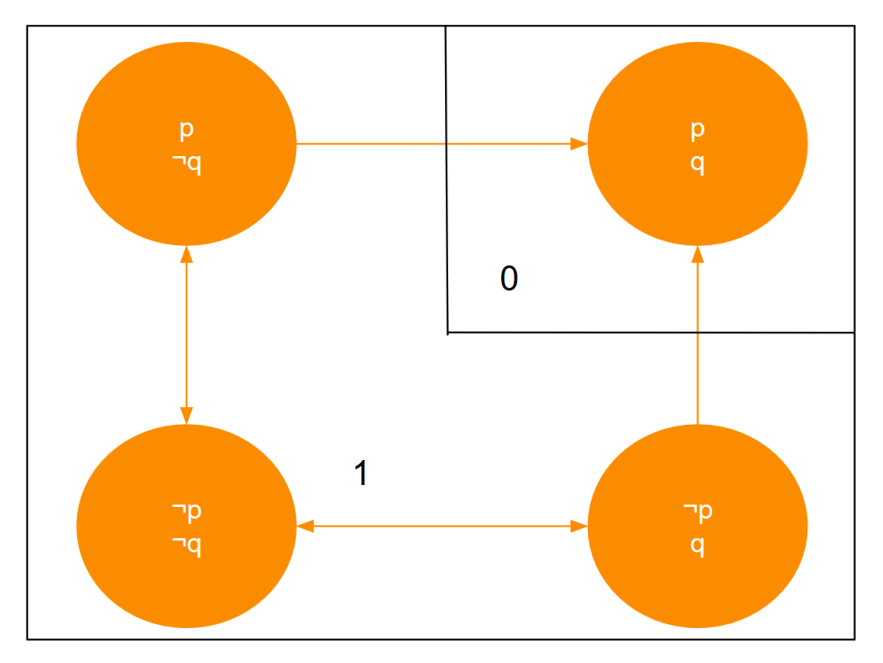
\includegraphics[width=0.5\textwidth]{slide19.eps}
  \caption{Before $(\phi \to \neg \rho)$ announcement, with the derived Spohn rank of states}
\end{figure}

\begin{figure}[h]
  \centering
  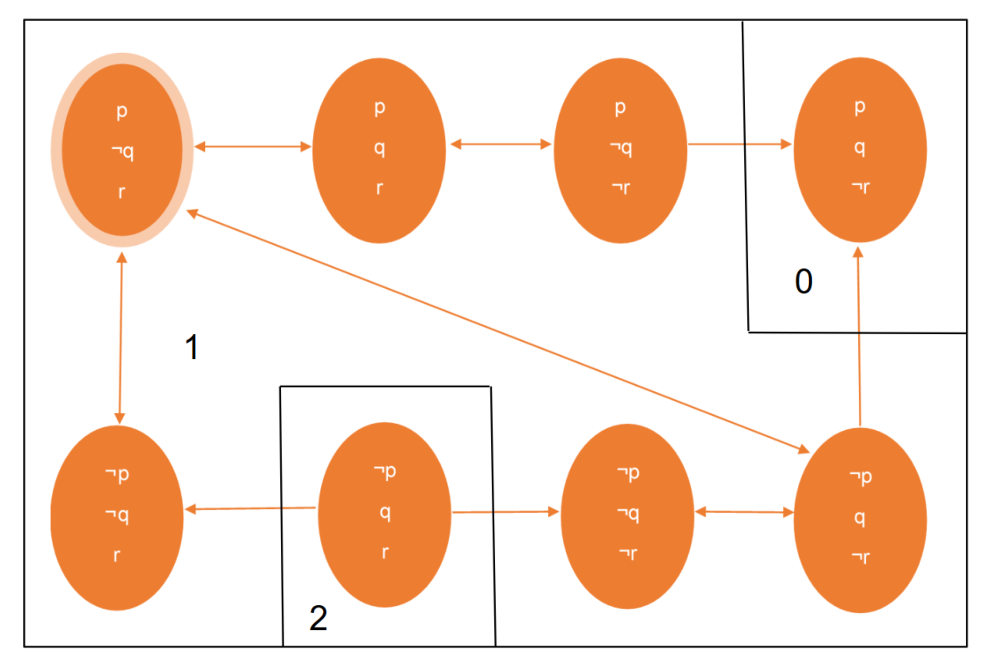
\includegraphics[width=0.5\textwidth]{slide21.eps}
  \caption{After $(\phi \to \neg \rho)$ announcement, with the derived Spohn rank of states}
\end{figure}

\section{Non-Gettier Types}
What if you aren't a Gettier Truth-teller? Negating the necessary conditions of Gettier Truth-tellers gives rise to 3 other possible cases when the state of the actual world remains the same. These cases give insight on what other kinds of truth tellers or liars may exist and what might differentiate them.
\newpage
\section{The Beliefless Truth-teller}
$$((\neg \phi \wedge \psi) \wedge \neg B(\phi \to \psi) \wedge \neg B \phi)$$
In this case, the speaker has no belief in any of the Gettier conditions. The speaker may very well have other types of belief or knowledge that contribute to the announcement of $\psi$, but these are further sub-cases to be examined. If there is no other belief or knowledge that pertains to $\psi$, a speaker satisfying these conditions announces $\psi$ with no rationale or justification. The announcement happens to be true in this world, but that is pure happenstance (when discarding other possible beliefs or knowledge).\\
This case does allow for sub-cases in which the speaker does in fact have a justified true belief in $\psi$ however, as it allows for sub-cases such as:
$$((\neg \phi \wedge \psi) \wedge \neg B(\phi \to \psi) \wedge B \neg \phi)$$

\subsection{State Plausibility Models}
\quad
\newline \newline \newline
\begin{figure}[h!]
  \centering
  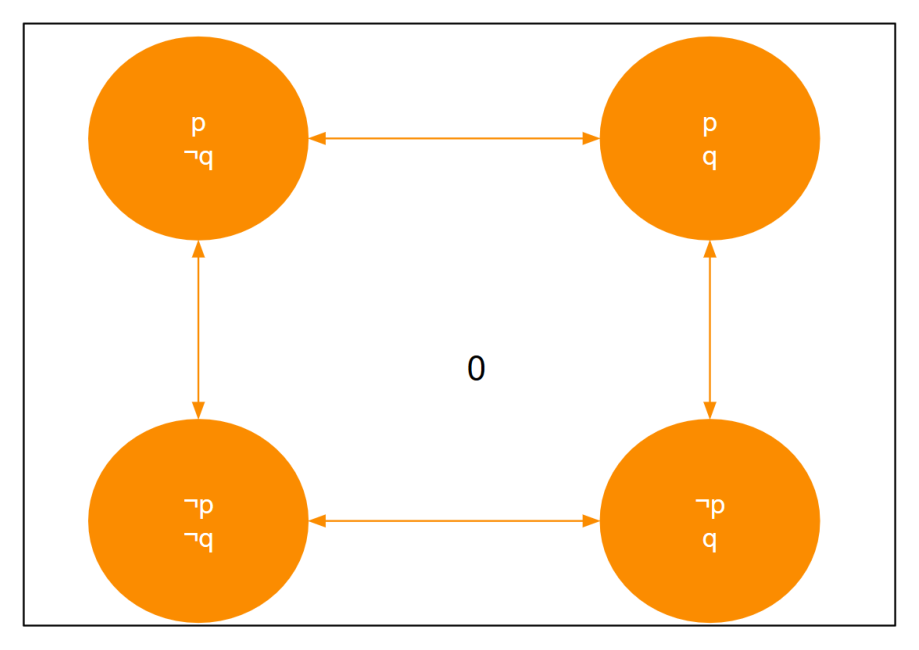
\includegraphics[width=0.5\textwidth]{slide25.eps}
  \caption{Before $(\phi \to \neg \rho)$ announcement, with the derived Spohn rank of states}
\end{figure}
\newline \newline \newline
\begin{figure}[h!]
  \centering
  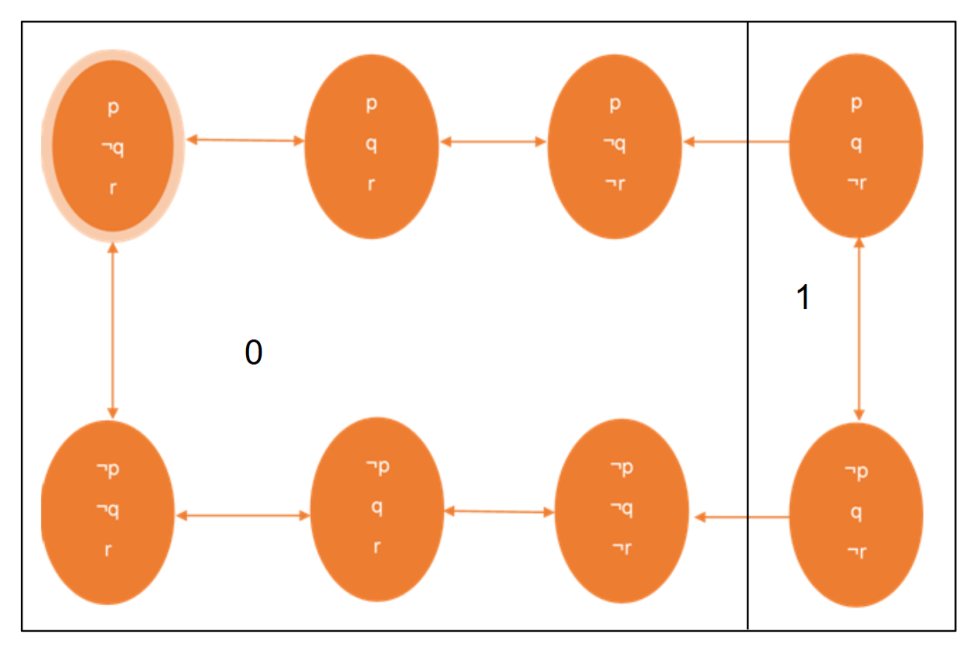
\includegraphics[width=0.5\textwidth]{slide27.eps}
  \caption{After $(\phi \to \neg \rho)$ announcement, with the derived Spohn rank of states}
\end{figure}
\quad
\newline

\section{The Uninformed Accidental Truth-teller}
$$((\neg \phi \wedge \psi) \wedge \neg B(\phi \to \psi) \wedge B \phi)$$
In this case, one has an untrue belief about the world ($B\phi$ when $\neg \phi$), but also doesn't have a belief in the implication $(\phi \to \psi)$ that Gettier Truth Tellers have (a belief which holds true in reality in this state of the world). If one announces $\psi$ with these conditions, they are announcing a true thing but have very little rationale in doing so without considering additional beliefs. They are indifferent on $\psi$ if no other beliefs are held, and therefore announcing $\psi$ seems to be announcing something insincerely. One possible sub-case:
\begin{align*}
&((\neg \phi \wedge \psi) \wedge \neg B(\phi \to \psi) \wedge B \phi \wedge B \neg (\phi \to \psi ))\\
\leftrightarrow &((\neg \phi \wedge \psi) \wedge \neg B(\phi \to \psi) \wedge B \phi \wedge B (\phi \wedge \neg \psi ))\\
\leftrightarrow &((\neg \phi \wedge \psi) \wedge \neg B(\phi \to \psi) \wedge B \phi \wedge B \neg \psi)
\end{align*}
This sub-case is one in which the speaker announcing $\psi$ announces something true about the world, but does so by saying something she believes to be untrue - implying an intent to deceive and a type of lie, but announcing a true statement due to her incorrect beliefs. 
\newpage
\subsection{State Plausibility Models}
\quad
\newline
\begin{figure}[h!]
  \centering
  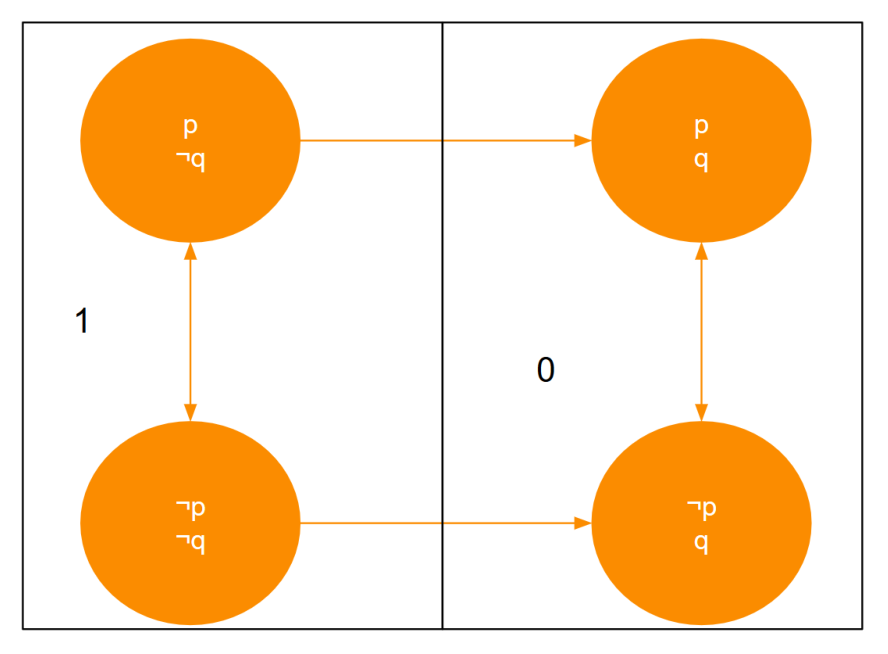
\includegraphics[width=0.5\textwidth]{slide30.eps}
  \caption{Before $(\phi \to \neg \rho)$ announcement, with the derived Spohn rank of states}
\end{figure}
\begin{figure}[h!]
  \centering
  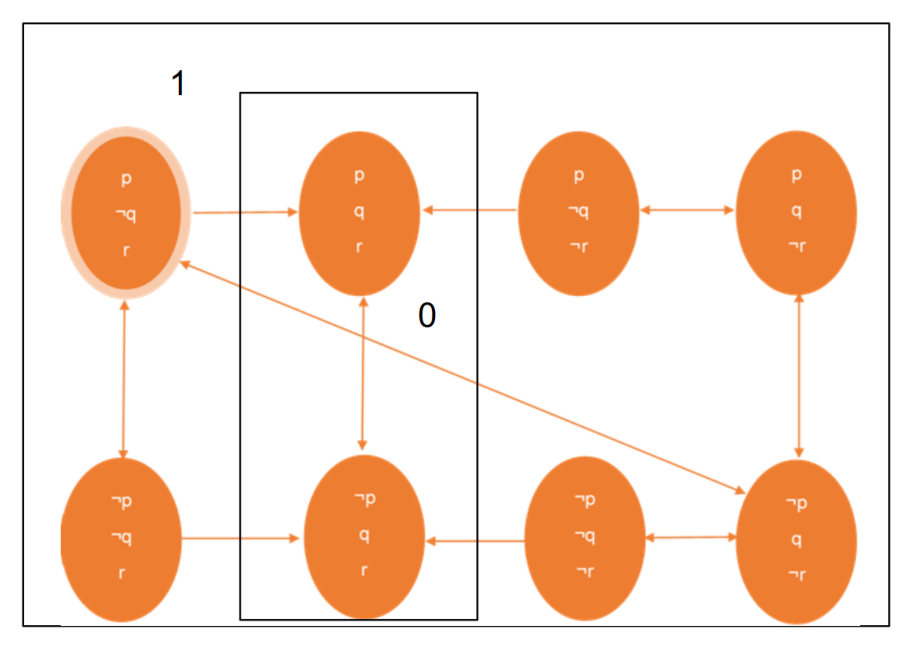
\includegraphics[width=0.5\textwidth]{slide32.eps}
  \caption{After $(\phi \to \neg \rho)$ announcement, with the derived Spohn rank of states}
\end{figure}
\quad
\newline

\section{The Accurate Believer}
$$(\neg \phi \wedge \psi) \wedge B(\phi \to \psi) \wedge \neg B \phi)$$
In this case, announcing $\psi$ is again saying something true, but based on very little evidence without considering other beliefs the speaker may hold. They don’t believe $\phi$, but they do believe $(\phi \to \psi)$, and announcing $\psi$ may be with the intent to deceive if they don't believe $\psi$. This case is one in which the speaker has the most accurate set of beliefs. It is the only case in which the speaker both believes the true statement $(\phi \to \psi)$ and does not falsely believe $\phi$. Interestingly, this case is the only one in which Spohn Rank 0 contains only 5 cases rather than 6. This case allows for sub-cases in which the speaker has a justified true belief of $\psi$ or a justified false belief in $\neg \psi$.

$$(\neg \phi \wedge \psi) \wedge B(\phi \to \psi) \wedge \neg B \phi \wedge B(\psi \to \phi))$$
In this case, one cannot be sincere in announcing $\psi$ as it would then result in $B\phi$ but it is given that $\neg B \phi$
\newpage
\subsection{State Plausibility Models}
\quad
\newline
\begin{figure}[h!]
  \centering
  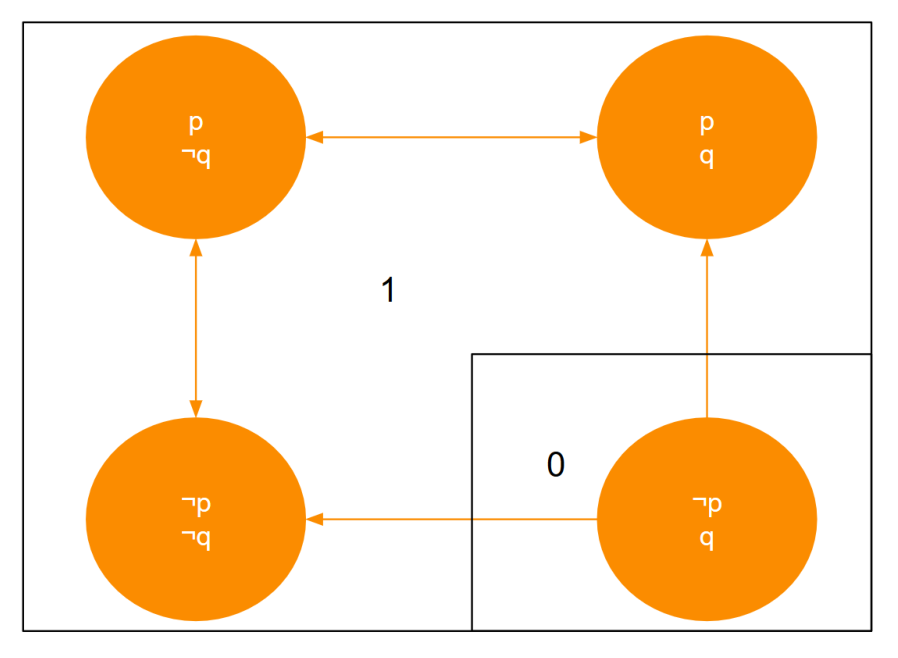
\includegraphics[width=0.5\textwidth]{slide34.eps}
  \caption{Before $(\phi \to \neg \rho)$ announcement, with the derived Spohn rank of states}
\end{figure}
\begin{figure}[h!]
  \centering
  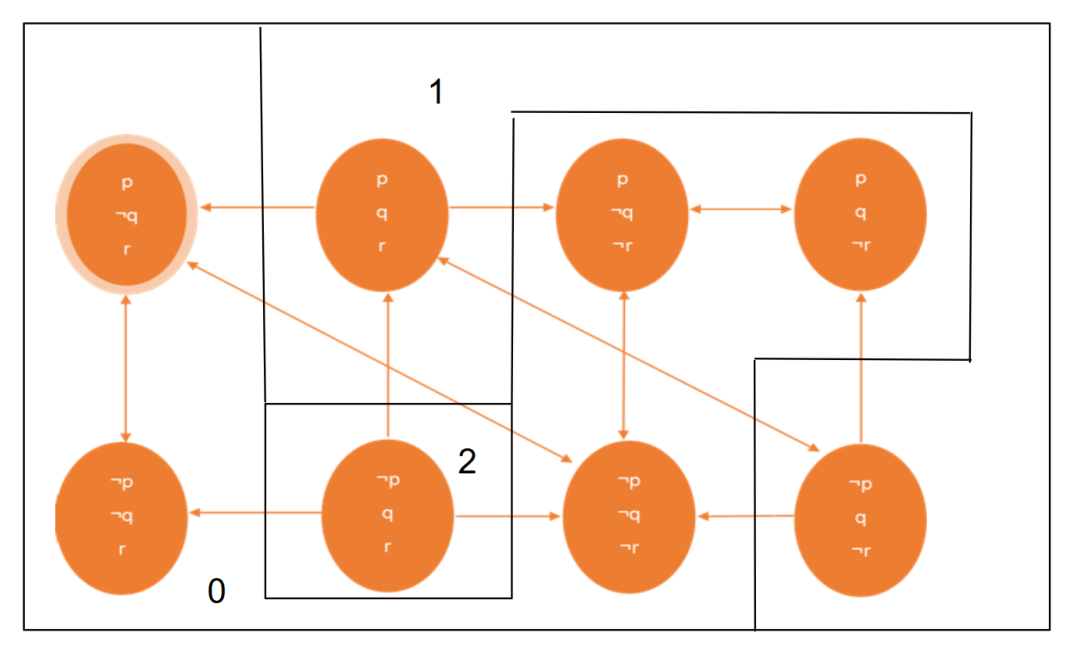
\includegraphics[width=0.5\textwidth]{slide36.eps}
  \caption{After $(\phi \to \neg \rho)$ announcement, with the derived Spohn rank of states}
\end{figure}
\quad
\newline

\chapter{Why is a Raven like a Writing Desk?: Reflections and Suggestions for Further Work}
\section{Reflections}
Throughout this project, one of our greatest challenges seemed to be in delineating a specific, narrow focus. We ended up expanding some problems rather than reducing them (e.g. considering the notion of justification ended up giving rise to more questions than answers). We would have liked to go into greater detail with computational aspects and evaluate if this sort of framework has use beyond a thought experiment. We would have probably benefited from choosing a broad topic and working to narrow it down rather than starting from a specific notion of pre-conditions and their relation to lying and truth-telling (inspired by a brief section in Johan van Benthem’s Logical Dynamics of Information and Interaction)\autocite{BenthemJohanvan2011Ldoi} and expanding it outwards. Despite this challenge, we believe the content put forth in this paper is of strong conceptual use.
\newpage
\section{Suggestions for Further Work}
Meta:
\begin{itemize}
\item Is there an exhaustive list of liars and truth-tellers?
\item Is it even possible to arrive at one at all?
\end{itemize}
Basic Types:
\begin{itemize}
\item Interactions between omniscient and insincere men
\item How different thresholds affect what can be claimed by sincere and insincere men ($\tau \leq \frac{1}{2}$ and $\tau > \frac{1}{2}$)
\end{itemize}
Building on Gettier and non-Gettier Types:
\begin{itemize}
\item What sub-cases arise from the non-Gettier cases?\item What facets of interaction with these different sub-case agents will differ?
\item Is this non-Gettier approach a useful approach or is too much redundancy embedded in it?
\end{itemize}

\printbibliography
\end{document}
